\documentclass{ximera}

%\usepackage{todonotes}

\newcommand{\todo}{}

\usepackage{tkz-euclide}
\tikzset{>=stealth} %% cool arrow head
\tikzset{shorten <>/.style={ shorten >=#1, shorten <=#1 } } %% allows shorter vectors

\usepackage{tkz-tab}  %% sign charts
\usetikzlibrary{decorations.pathreplacing} 

\usetikzlibrary{backgrounds} %% for boxes around graphs
\usetikzlibrary{shapes,positioning}  %% Clouds and stars
\usetikzlibrary{matrix} %% for matrix
\usepgfplotslibrary{polar} %% for polar plots
\usetkzobj{all}
\usepackage[makeroom]{cancel} %% for strike outs
%\usepackage{mathtools} %% for pretty underbrace % Breaks Ximera
\usepackage{multicol}

\usepackage{polynom}



\usepackage[many]{tcolorbox}  %% for titled boxes
\newtcolorbox{xbox}[1]{%
    tikznode boxed title,
    enhanced,
    arc=0mm,
    interior style={white},
    attach boxed title to top center= {yshift=-\tcboxedtitleheight/2},
    fonttitle=\bfseries,
    colbacktitle=white,coltitle=black,
    boxed title style={size=normal,colframe=white,boxrule=0pt},
    title={#1}}


\usepackage{array}
\setlength{\extrarowheight}{+.1cm}   
\newdimen\digitwidth
\settowidth\digitwidth{9}
\def\divrule#1#2{
\noalign{\moveright#1\digitwidth
\vbox{\hrule width#2\digitwidth}}}





\newcommand{\RR}{\mathbb R}
\newcommand{\R}{\mathbb R}
\newcommand{\N}{\mathbb N}
\newcommand{\Z}{\mathbb Z}

%\renewcommand{\d}{\,d\!}
\renewcommand{\d}{\mathop{}\!d}
\newcommand{\dd}[2][]{\frac{\d #1}{\d #2}}
\newcommand{\pp}[2][]{\frac{\partial #1}{\partial #2}}
\renewcommand{\l}{\ell}
\newcommand{\ddx}{\frac{d}{\d x}}
\newcommand{\ddt}{\frac{d}{\d t}}

\newcommand{\zeroOverZero}{\ensuremath{\boldsymbol{\tfrac{0}{0}}}}
\newcommand{\inftyOverInfty}{\ensuremath{\boldsymbol{\tfrac{\infty}{\infty}}}}
\newcommand{\zeroOverInfty}{\ensuremath{\boldsymbol{\tfrac{0}{\infty}}}}
\newcommand{\zeroTimesInfty}{\ensuremath{\small\boldsymbol{0\cdot \infty}}}
\newcommand{\inftyMinusInfty}{\ensuremath{\small\boldsymbol{\infty - \infty}}}
\newcommand{\oneToInfty}{\ensuremath{\boldsymbol{1^\infty}}}
\newcommand{\zeroToZero}{\ensuremath{\boldsymbol{0^0}}}
\newcommand{\inftyToZero}{\ensuremath{\boldsymbol{\infty^0}}}



\newcommand{\numOverZero}{\ensuremath{\boldsymbol{\tfrac{\#}{0}}}}
\newcommand{\dfn}{\textbf}
%\newcommand{\unit}{\,\mathrm}
\newcommand{\unit}{\mathop{}\!\mathrm}
\newcommand{\eval}[1]{\bigg[ #1 \bigg]}
\newcommand{\seq}[1]{\left( #1 \right)}
\renewcommand{\epsilon}{\varepsilon}
\renewcommand{\iff}{\Leftrightarrow}

\DeclareMathOperator{\arccot}{arccot}
\DeclareMathOperator{\arcsec}{arcsec}
\DeclareMathOperator{\arccsc}{arccsc}
\DeclareMathOperator{\si}{Si}
\DeclareMathOperator{\proj}{proj}
\DeclareMathOperator{\scal}{scal}


\newcommand{\tightoverset}[2]{% for arrow vec
  \mathop{#2}\limits^{\vbox to -.5ex{\kern-0.75ex\hbox{$#1$}\vss}}}
\newcommand{\arrowvec}[1]{\tightoverset{\scriptstyle\rightharpoonup}{#1}}
\renewcommand{\vec}{\mathbf}
\newcommand{\veci}{\vec{i}}
\newcommand{\vecj}{\vec{j}}
\newcommand{\veck}{\vec{k}}
\newcommand{\vecl}{\boldsymbol{\l}}

\newcommand{\dotp}{\bullet}
\newcommand{\cross}{\boldsymbol\times}
\newcommand{\grad}{\boldsymbol\nabla}
\newcommand{\divergence}{\grad\dotp}
\newcommand{\curl}{\grad\cross}
%\DeclareMathOperator{\divergence}{divergence}
%\DeclareMathOperator{\curl}[1]{\grad\cross #1}


\colorlet{textColor}{black} 
\colorlet{background}{white}
\colorlet{penColor}{blue!50!black} % Color of a curve in a plot
\colorlet{penColor2}{red!50!black}% Color of a curve in a plot
\colorlet{penColor3}{red!50!blue} % Color of a curve in a plot
\colorlet{penColor4}{green!50!black} % Color of a curve in a plot
\colorlet{penColor5}{orange!80!black} % Color of a curve in a plot
\colorlet{fill1}{penColor!20} % Color of fill in a plot
\colorlet{fill2}{penColor2!20} % Color of fill in a plot
\colorlet{fillp}{fill1} % Color of positive area
\colorlet{filln}{penColor2!20} % Color of negative area
\colorlet{fill3}{penColor3!20} % Fill
\colorlet{fill4}{penColor4!20} % Fill
\colorlet{fill5}{penColor5!20} % Fill
\colorlet{gridColor}{gray!50} % Color of grid in a plot

\newcommand{\surfaceColor}{violet}
\newcommand{\surfaceColorTwo}{redyellow}
\newcommand{\sliceColor}{greenyellow}




\pgfmathdeclarefunction{gauss}{2}{% gives gaussian
  \pgfmathparse{1/(#2*sqrt(2*pi))*exp(-((x-#1)^2)/(2*#2^2))}%
}


%%%%%%%%%%%%%
%% Vectors
%%%%%%%%%%%%%

%% Simple horiz vectors
\renewcommand{\vector}[1]{\left\langle #1\right\rangle}


%% %% Complex Horiz Vectors with angle brackets
%% \makeatletter
%% \renewcommand{\vector}[2][ , ]{\left\langle%
%%   \def\nextitem{\def\nextitem{#1}}%
%%   \@for \el:=#2\do{\nextitem\el}\right\rangle%
%% }
%% \makeatother

%% %% Vertical Vectors
%% \def\vector#1{\begin{bmatrix}\vecListA#1,,\end{bmatrix}}
%% \def\vecListA#1,{\if,#1,\else #1\cr \expandafter \vecListA \fi}

%%%%%%%%%%%%%
%% End of vectors
%%%%%%%%%%%%%

%\newcommand{\fullwidth}{}
%\newcommand{\normalwidth}{}



%% makes a snazzy t-chart for evaluating functions
%\newenvironment{tchart}{\rowcolors{2}{}{background!90!textColor}\array}{\endarray}

%%This is to help with formatting on future title pages.
\newenvironment{sectionOutcomes}{}{} 



%% Flowchart stuff
%\tikzstyle{startstop} = [rectangle, rounded corners, minimum width=3cm, minimum height=1cm,text centered, draw=black]
%\tikzstyle{question} = [rectangle, minimum width=3cm, minimum height=1cm, text centered, draw=black]
%\tikzstyle{decision} = [trapezium, trapezium left angle=70, trapezium right angle=110, minimum width=3cm, minimum height=1cm, text centered, draw=black]
%\tikzstyle{question} = [rectangle, rounded corners, minimum width=3cm, minimum height=1cm,text centered, draw=black]
%\tikzstyle{process} = [rectangle, minimum width=3cm, minimum height=1cm, text centered, draw=black]
%\tikzstyle{decision} = [trapezium, trapezium left angle=70, trapezium right angle=110, minimum width=3cm, minimum height=1cm, text centered, draw=black]


\outcome{Understand the statement of the Extreme Value Theorem.}

\title[Dig-In:]{The Extreme Value Theorem}

\begin{document}
\begin{abstract}
  We examine a fact about continuous functions.
\end{abstract}
\maketitle

\begin{definition}\hfil\index{maximum/minimum!absolute}
\begin{enumerate}
\item A function $f$ has a \dfn{global maximum} at $x=a$, if $f(a)\ge
  f(x)$ for every $x$ in the domain of the function.
\item A function $f$ has a \dfn{global minimum} at $x=a$, if $f(a)\le
  f(x)$ for every $x$ in the domain of the function.
\end{enumerate} 
A \dfn{global extremum}\index{extremum!global} is either a
global maximum or a global minimum.
\end{definition}

Let $f$ be the function given by the graph below. 
\begin{image}
  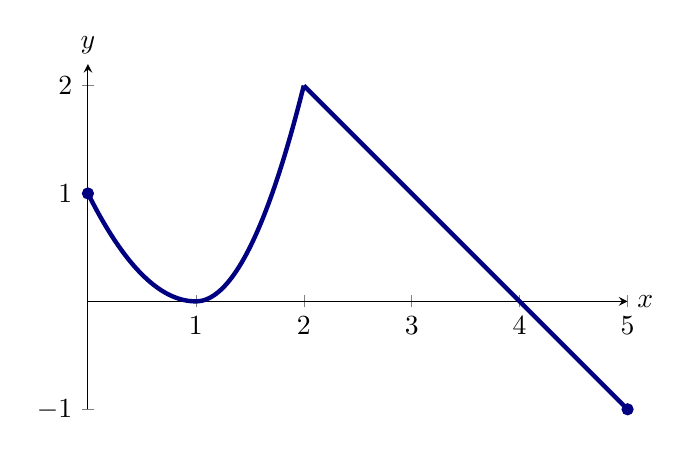
\begin{tikzpicture}
    \begin{axis}[
            xmin=0, xmax=5, ymin=-1,ymax=2.2,
            unit vector ratio*=1 1 1,
            axis lines =middle, xlabel=$x$, ylabel=$y$,
            every axis y label/.style={at=(current axis.above origin),anchor=south},
            every axis x label/.style={at=(current axis.right of origin),anchor=west},
            xtick={0,...,5}, ytick={-1,...,2},
          ]
        \addplot[ultra thick, color=penColor, smooth, domain=(0:1)] {(x-1)^2};
        \addplot[ultra thick, color=penColor, smooth, domain=(1:2)] {2*(x-1)^2};
        \addplot[ultra thick, color=penColor, smooth, domain=(2:5)] {4-x};
	\addplot [color=penColor,fill=penColor,only marks,mark=*] coordinates{(0,1)};
	\addplot [color=penColor,fill=penColor,only marks,mark=*] coordinates{(5,-1)};
	
    \end{axis}
\end{tikzpicture}
\end{image}
\begin{question}
%%\author{Nela Lakos}
  Find the $x$-coordinate of the point where the function $f$ has a global maximum.
    \begin{prompt}
  \[
 x= \answer[given]{2}
  \]
  \end{prompt}
 
 Observe that $f(2)\ge f(x)$ for all $x$ in the domain of $f$. Notice, that the function $f$  has also a local maximum at $x=2$. 
 
 \begin{question}
 %%\author{Nela Lakos}

   Find the $x$-coordinate of the point where the function $f$ has a
   global minimum.
   \begin{prompt}
     \[
     x= \answer[given]{5}
     \]
   \end{prompt}
   Observe that $f(5)\le f(x)$ for all $x$ in the domain of $f$. Notice, that the function $f$  does not have a local minimum at $x=5$. 
   Recall, a function cannot not have a local extremum  at a boundary point.
 \end{question}
 \begin{question}
   %%\author{Nela Lakos}
   Find the $x$-coordinate(s) of the point(s) where the function $f$ has a local minimum.
   \begin{prompt}
     \[
     x= \answer[given]{1}
  \]
   \end{prompt}
   Observe that $f(1)\le f(x)$ for all $x$ in the interval $(0,2)$. But it is not true that $f(1)\le f(x)$ for all $x$ in the domain of $f$. For example, $f(4.5)<f(1)$.
 \end{question}
\end{question}
\begin{question}
  Does every function attain a global extremum on its domain? Select the correct answer.
  \begin{multipleChoice}
    
    \choice{All functions must attain both global minimum and global maximum on their domain.}
 \choice{All functions  attain a global minimum on their domain.}
 \choice{All functions  attain a global maximum on their domain.}
 \choice[correct]{Some functions have no global extremums on their domain.}
  \end{multipleChoice}
 
\end{question}
Check the following graph.
\begin{image}
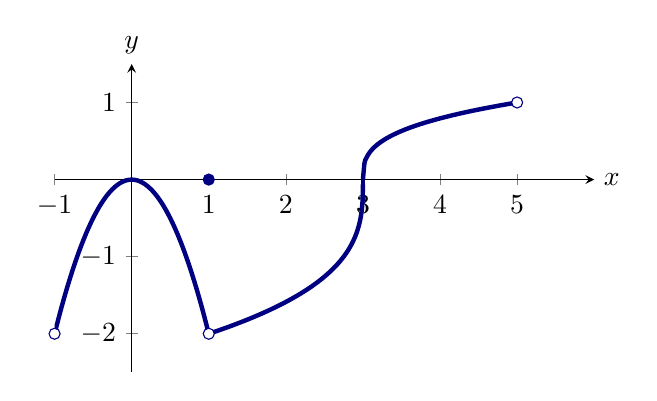
\begin{tikzpicture}
    \begin{axis}[
            xmin=-1, xmax=6, ymin=-2.5,ymax=1.5,
            unit vector ratio*=1 1 1,
            axis lines =middle, xlabel=$x$, ylabel=$y$,
            every axis y label/.style={at=(current axis.above origin),anchor=south},
            every axis x label/.style={at=(current axis.right of origin),anchor=west},
            xtick={-1,...,5}, ytick={-2,...,1},
          ]
        \addplot[ultra thick, color=penColor, smooth, domain=(-1:1)] {-2*x^2};
        \addplot[ultra thick, color=penColor, smooth, samples=500, domain=(1:3)] {-2*2^(-1/3)*(3-x)^(1/3)};
	\addplot[ultra thick, color=penColor, smooth, samples=100, domain=(3:5)] {2^(-1/3)*(x-3)^(1/3)};
	\addplot[ultra thick, color=penColor, smooth]plot coordinates{(3,-.1) (3,0)};
	\addplot [color=penColor,fill=background,only marks,mark=*] coordinates{(-1,-2)};
	\addplot [color=penColor,fill=background,only marks,mark=*] coordinates{(5,1)};
          \addplot[color=penColor,fill=background,only marks, mark=*] coordinates{(1,-2)};
          \addplot [color=penColor,fill=penColor,only marks,mark=*] coordinates{(1,0)};
    \end{axis}
\end{tikzpicture}
\end{image}
Notice, the function is \textbf{not continuous} at $x=1$, and, therefore, $f$ is \textbf{not continuous}  on its domain, $(-1,5)$.\\
Does the function attain a global extremum on its domain? Select the correct answer.
 \begin{multipleChoice}
%%\author{Nela Lakos}

 \choice{The function attains both global minimum and global maximum on its domain.}
 \choice{The function attains a global minimum, but has no global maximum on its domain.}
 \choice{The function attains a global maximum, but has no global minimum on its domain.}
 \choice [correct]{The function has no global extremum on its domain.}
  \end{multipleChoice}
  Check the following graph.
\begin{image}
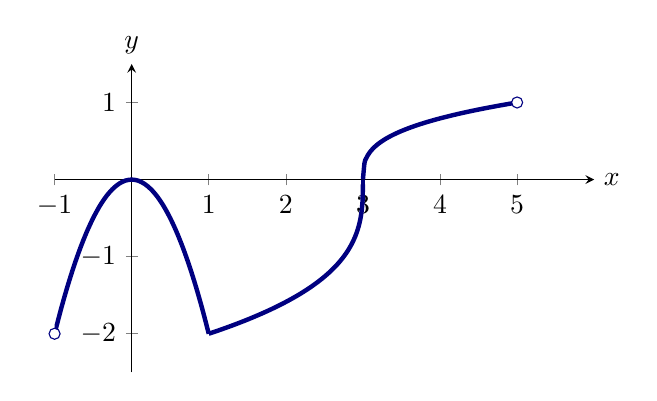
\begin{tikzpicture}
    \begin{axis}[
            xmin=-1, xmax=6, ymin=-2.5,ymax=1.5,
            unit vector ratio*=1 1 1,
            axis lines =middle, xlabel=$x$, ylabel=$y$,
            every axis y label/.style={at=(current axis.above origin),anchor=south},
            every axis x label/.style={at=(current axis.right of origin),anchor=west},
            xtick={-1,...,5}, ytick={-2,...,1},
          ]
        \addplot[ultra thick, color=penColor, smooth, domain=(-1:1)] {-2*x^2};
        \addplot[ultra thick, color=penColor, smooth, samples=500, domain=(1:3)] {-2*2^(-1/3)*(3-x)^(1/3)};
	\addplot[ultra thick, color=penColor, smooth, samples=100, domain=(3:5)] {2^(-1/3)*(x-3)^(1/3)};
	\addplot[ultra thick, color=penColor, smooth]plot coordinates{(3,-.1) (3,0)};
	\addplot [color=penColor,fill=background,only marks,mark=*] coordinates{(-1,-2)};
	\addplot [color=penColor,fill=background,only marks,mark=*] coordinates{(5,1)};
	
    
       
    \end{axis}
\end{tikzpicture}
\end{image}
Notice, the function is \textbf{continuous} on its domain $(-1,5)$.
Does the function given by the graph above attain a global extremum on its domain? Select the correct answer.
 \begin{multipleChoice}
%%\author{Nela Lakos}

 \choice{The function attains both global minimum and global maximum on its domain.}
 \choice[correct]{ The function attains a global minimum, but has no global maximum on its domain.}
 \choice{The function attains a global maximum, but has no global minimum on its domain.}
 \choice {The function has no global extremum on its domain.}
  \end{multipleChoice}
   Check the following graph.
\begin{image}
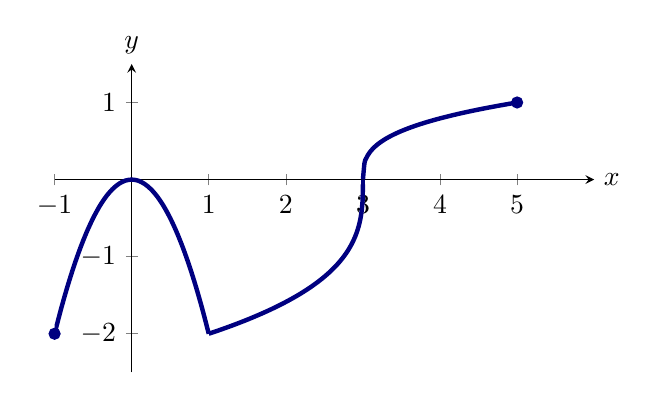
\begin{tikzpicture}
    \begin{axis}[
            xmin=-1, xmax=6, ymin=-2.5,ymax=1.5,
            unit vector ratio*=1 1 1,
            axis lines =middle, xlabel=$x$, ylabel=$y$,
            every axis y label/.style={at=(current axis.above origin),anchor=south},
            every axis x label/.style={at=(current axis.right of origin),anchor=west},
            xtick={-1,...,5}, ytick={-2,...,1},
          ]
        \addplot[ultra thick, color=penColor, smooth, domain=(-1:1)] {-2*x^2};
        \addplot[ultra thick, color=penColor, smooth, samples=500, domain=(1:3)] {-2*2^(-1/3)*(3-x)^(1/3)};
	\addplot[ultra thick, color=penColor, smooth, samples=100, domain=(3:5)] {2^(-1/3)*(x-3)^(1/3)};
	\addplot[ultra thick, color=penColor, smooth]plot coordinates{(3,-.1) (3,0)};
	\addplot [color=penColor,fill=penColor,only marks,mark=*] coordinates{(-1,-2)};
		\addplot [color=penColor,fill=penColor,only marks,mark=*] coordinates{(5,1)};

    
       
    \end{axis}
\end{tikzpicture}
\end{image}
Notice, the function is \textbf{continuous on a closed interval} $[-1,5]$.
Does the function given by the graph above attain a global extremum on its domain? Select the correct answer.
\begin{multipleChoice}
%%\author{Nela Lakos}

 \choice[correct]{ The function attains both global minimum and global maximum on its domain.}
 \choice{The function attains a global minimum, but has no global maximum on its domain.}
 \choice{The function attains a global maximum, but has no global minimum on its domain.}
 \choice {The function has no global extremum on its domain.}
  \end{multipleChoice}
\begin{question}
%%\author{Nela Lakos}

  Find the x-coordinate(s) of the point(s) where the function $f$ has a global minimum.
    \begin{prompt}
  \[
 x= \answer[given]{-1},      x= \answer[given]{1}
  \]
  \end{prompt}
 \end{question}
 \begin{question}
  Find the x-coordinate(s) of the point(s) where the function $f$ has a global maximum.
    \begin{prompt}
  \[
 x= \answer[given]{5}
  \]
  \end{prompt}
 \end{question}
Sometimes it is important to know whether a function attains a global extremum on its domain. 
The last three examples suggest the following theorem. 

\begin{theorem}[Extreme Value Theorem]\label{theorem:evt}\index{Extreme Value Theorem}
If $f$ is a continuous function for all $x$ in the closed interval
$[a,b]$, then there are points $c$ and $d$ in $[a,b]$, such that
$(c,f(c))$ is a global maximum and $(d,f(d))$ is a global
minimum on $[a, b]$.

Below, we see a geometric interpretation of this theorem.
\begin{image}
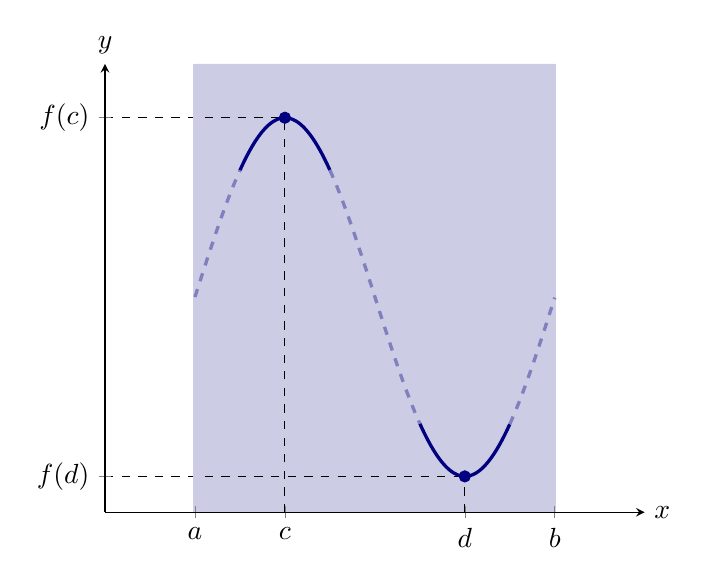
\begin{tikzpicture}
	\begin{axis}[
            domain=0:6, xmin=0, xmax=6, ymin=0, ymax=2.5,
            axis lines =left, xlabel=$x$, ylabel=$y$,
            every axis y label/.style={at=(current axis.above origin),anchor=south},
            every axis x label/.style={at=(current axis.right of origin),anchor=west},
            xtick={1,2,4,5}, ytick={.2,2.2},
            xticklabels={$a$,$c$,$d$,$b$}, yticklabels={$f(d)$,$f(c)$},
            axis on top,
          ]
          \addplot [draw=none, fill=fill1, domain=(1:5)] {2.5} \closedcycle;

          \addplot [textColor,dashed] plot coordinates {(0,2.2) (2,2.2)};
          \addplot [textColor,dashed] plot coordinates {(0,.2) (4,.2)};
          \addplot [textColor,dashed] plot coordinates {(2,0) (2,2.2)};
          \addplot [textColor,dashed] plot coordinates {(4,0) (4,.2)};

          \addplot [fill1,very thick] plot coordinates {(1,0) (1,2.5)};
          \addplot [fill1,very thick] plot coordinates {(5,0) (5,2.5)};

          \addplot [very thick,penColor, smooth,domain=(1.5:2.5)] {sin(deg(x*1.57-1.57)) + 1.2};%max
          \addplot [very thick,penColor, smooth,domain=(3.5:4.5)] {sin(deg(x*1.57-1.57)) + 1.2};%min
          \addplot [very thick,dashed,penColor!50!background, smooth,domain=(2.5:3.5)] {sin(deg(x*1.57 - 1.57)) + 1.2}; 
          \addplot [very thick,dashed,penColor!50!background, smooth,domain=(1:1.5)] {sin(deg(x*1.57 - 1.57)) + 1.2}; 
          \addplot [very thick,dashed,penColor!50!background, smooth,domain=(4.5:5)] {sin(deg(x*1.57 - 1.57)) + 1.2}; 
          
          \addplot [color=penColor,fill=penColor,only marks,mark=*] coordinates{(2,2.2)};  %% closed hole          
          \addplot [color=penColor,fill=penColor,only marks,mark=*] coordinates{(4,.2)};  %% closed hole          
        \end{axis}
\end{tikzpicture}
%% \caption{A geometric interpretation of the Extreme Value Theorem. A
%%   continuous function $f(x)$ attains both an global maximum and an
%%   global minimum on an interval $[a,b]$. Note, it may be the case
%%   that $a=c$, $b=d$, or that $d<c$.}
%% \label{figure:extreme-value}
%% \end{marginfigure}
\end{image}
\end{theorem}
\begin{question}
  Would this theorem hold if we were working on an open interval?
  \begin{multipleChoice}
    \choice{yes}
    \choice[correct]{no}
  \end{multipleChoice}
  \begin{hint}
    Consider $\tan(\theta)$ for $-\pi/2 < \theta < \pi/2$. Does this function achieve its maximum and minimum? 
  \end{hint}
\end{question}

\begin{question}%%\author{Nela Lakos}
  Would this theorem hold if we were working on a closed interval
  $[a,b]$, but a function is not continuous on $[a,b]$?
  \begin{prompt}
    \begin{multipleChoice}
      \choice{yes}
      \choice[correct]{no}
    \end{multipleChoice}
    \begin{hint}
      Consider a function $f$ on a closed interval $[-1,1]$, defined
      by $f(x)=\frac{1}{x}$ for $x\neq 0$ and $f(0)=0$ . Does this
      function achieve its maximum and minimum?
    \end{hint}
  \end{prompt}
\end{question}

Assume that a function $f$ is continuous on a closed interval
$[a,b]$. By the Extreme Value Theorem, $f$ attains both global
extremums on the interval $[a,b]$.  How can we locate these global
extrema? We have seen that they can occur at the end points or in the
open interval $(a,b)$.  If a global extremum occurs at a point $x$ in
the open interval $(a,b)$, then $f$ has a local extremum at $x$. That
means that $f$ has a critical point at $x$.  So, the global extrema of
a function $f$ occur either at the end points, $a$ or $b$, or at
critical points. If we want to locate the global extrema, we have to
evaluate the function at the end points and at critical points, and
compare the values.



\begin{example}
	Find the extreme values of $f(x) = x^3 - 3x^2 - 1$ on the interval $[-1,4]$.
	\begin{explanation}
		The derivative is $f'(x) = 3x^2 - 6x$  
			\begin{align*}
				f'(x) &= 0\\
				3x^2 - 6x &= 0\\
				3x(x-2) &= 0
			\end{align*}
			The critical points are $x=0$ and $x=2$ (both these lie in $(-1,4)$), 
			with values $f(0) = -1$ and  $f(2) = -5$.
			
			The endpoints have values $f(-1) = -5$ and $f(4) = 15$.
			
			That gives us a list of values $\{ -1, -5, 15\}$.
			
			The global maximum value of $f$ is $15$ (occurring at $x=4$) and a 
			global minimum value of $-5$ (occurring at $x=-1$ and $x=2$).
	\end{explanation}
\end{example}

\begin{question}%%\author{Nela Lakos}
Let $f(x)=x^2e^{-x}$, for $ -2\le x\le1$. Locate the global extremums
of $f$ on the closed interval $[-2,1]$. Does the function $f$ satisfy
the conditions of the Extreme Value Theorem on its domain?
 \begin{multipleChoice}
   \choice{Yes, because $f$ is continuous on $(-2,1)$.}
   \choice[correct]{Yes, because $f$ is continuous on $[-2,1]$.}
   \choice{No, because $f$ is  not continuous on $[-2,1]$.}
   \choice{No, because $f$ is  not differentiable on  $(-2,1)$.}
 \end{multipleChoice}
 Therefore, the Extreme Value Theorem guarantees that the function $f$
 attains both global extremums on its domain. The global extremums
 occur at the end points or at critical points.
  
 Find the critical points of $f$. First, compute the derivative of $f$.
 \begin{prompt}
   \[
   f'(x)= xe^{-x}(\answer[given]{2-x})
   \]
 \end{prompt}
 In order to find the critical points of $f$, we have to solve the
 equation
 \begin{prompt}
   \[
   f'(x)= \answer[given]{0}.
   \]
 \end{prompt}
 It follows that the function $f$ has only one critical point
 $\left(c,f(c)\right)$. Find $c$.
 \begin{prompt}
   \[
   c= \answer[given]{0}
   \]
 \end{prompt}
 In order to locate the global extremums of $f$, we have to evaluate
 $f$ at the end points and at the critical point.
 \begin{prompt}
   \[
   f(-2)= \answer[given]{4e^{2}}
   \]
 \end{prompt}
 \begin{prompt}
   \[
   f(c)= \answer[given]{0}
   \]
 \end{prompt}
 
 \begin{prompt}
   \[
   f(1)= \answer[given]{e^{-1}}
   \]
 \end{prompt}
 Order the three values, $f(-2)$, $f(c)$, and $f(1)$,  from smallest to largest. You should replace $c$ with its value, when you write $f(c)$  in your answer below.
 \begin{prompt}
  \[
  f(\answer[given]{0})<f(\answer[given]{1})<f(\answer[given]{-2})
  \]
  
 \end{prompt}
 
 Based on this comparison, find the location of the global minimum and global maximum of $f$. Circle the correct answer.
 \begin{multipleChoice}
   \choice{$f$ has a global maximum at $x=1$ and global minimum at $x=0$.}
   \choice{$f$ has a global maximum at $x=1$ and global minimum at $x=-2$.}
   \choice[correct]{ $f$ has a global maximum at $x=-2$ and global minimum at $x=0$.}
  \choice{$f$ has a global maximum at $x=-2$ and global minimum at $x=1$.}
  \choice{$f$ has a global maximum at $x=0$ and global minimum at $x=-2$.}
  \choice{$f$ has a global maximum at $x=0$ and global minimum at $x=1$.}
 \end{multipleChoice}
\end{question}


\begin{example}
	Find the extreme values of $g(x) = \sin(x) - \cos(x)$ on $[-\pi, \pi]$.
	\begin{explanation}
		To find critical points:
			\begin{align*}
				g'(x) &= 0\\
				\cos(x) + \sin(x) &= 0\\
				\cos(x)\left( 1 + \frac{\sin(x)}{\cos(x)} \right) &= 0\\
				\cos(x) \left( 1 + \tan(x) \right) &= 0
			\end{align*}
			Notice that $x$-values with $\cos(x) = 0$ have $\sin(x) = \pm 1$, so
			$g'(x) = 0 \pm 1 \neq 0$.  These values are not critical points.

			In the interval $[-\pi, \pi]$, the solutions of $\tan(x) = -1$ are 
			$x = -\frac{\pi}{4}, \frac{3\pi}{4}$.  (The solutions not in $(-\pi, \pi)$ are ignored.)
			\begin{align*}
				g\left( -\frac{\pi}{4} \right) &= \sin\left( -\frac{\pi}{4} \right) - \cos\left( -\frac{\pi}{4} \right)\\
					&= -\frac{1}{\sqrt{2}} - \frac{1}{\sqrt{2}}\\
					&= \answer[given]{-\sqrt{2}}\\
					\\
				g\left( \frac{3\pi}{4} \right) &= \sin\left( \frac{3\pi}{4} \right) - \cos\left( \frac{3\pi}{4} \right)\\
					&= \frac{1}{\sqrt{2}} + \frac{1}{\sqrt{2}}\\
					&= \answer[given]{\sqrt{2}}
			\end{align*}						
								
			The endpoints have values $g( -\pi ) = g(\pi) = \answer[given]{1}$
			
			The global maximum value of $g$ is $\answer[given]{\sqrt{2}}$ 
			(occurring at $x=\answer[given]{\frac{3\pi}{4}}$) and a 
			global minimum value of $\answer[given]{-\sqrt{2}}$ (occurring at $x=\answer[given]{\frac{\pi}{4} }$ ).
	\end{explanation}
\end{example}

\end{document}
